As the application launches, the first screen the user sees, in both versions, is the camera screen. The user must, in order to proceed further within the application, scan a QR code. Scanning a QR code is done by positioning the camera on the device (either Google Glass or smartphone) such that the QR code can be seen on screen. The user does not need to press any shutter button as the application automatically recognises the QR code pattern if seen on screen.%, as seen in Figure~\ref{}. The reasoning behind 

	\begin{figure}[ht!]
		\centering
		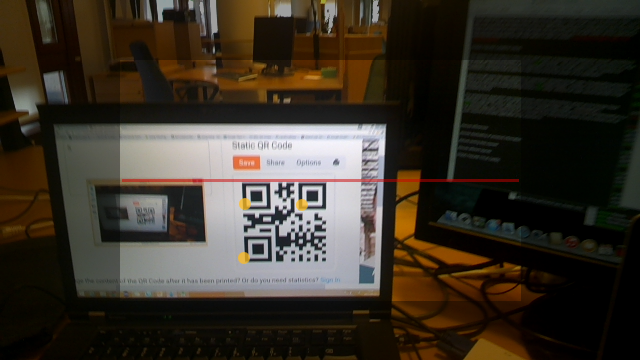
\includegraphics[width=110mm]{images/demo/qrCode}
		\caption{todo bild behöver uppdateras}
		\label{glassDemoQR}
	\end{figure}

The reason for not providing a menu on the start screen was because the application should be simple, easy to use and focus on what is important. Since the the focus of the application is to scan the QR code in order to receive the necessary instructions that is also the main focus of the first screen of the application.

When the QR code has been scanned the application decodes the QR code. The decoding process is done in the same way as described in Section~\ref{subsec:qrcode}. However, the decoding process is handled by the Zebra Crossing (ZXing) library~\cite{zxing}. ZXing is an open source barcode image processing library.

The smartphone application was based directly upon the ZXing library, where as the Google Glass application was based upon a port of the library to Google Glass, called ``BardcodeEye''~\cite{barcodeEye}. The main difference between ZXing and BarcodeEye is the fact that BarcodeEye is a full example application ready to be run, in contrast to the ZXing library which is only a library and as such needs to be attached to a runnable application.

The BarcodeEye application for Google Glass is however a bare bone application, used as an example and introduction as to how ZXing may be implemented in an application for Google Glass. BarcodeEye displayed the decoded information from the QR code and also gave the user the option to search the internet using the information previously decoded from the QR code.

As the QR code was intended to encode only a product ID, and the use the ID to download the instructions, rather than having all of the instructions encoded directly in the QR code the application had to be modified. However, prior to changing where the instructions were coming from the graphical layout of the application was changed. The change of layout was mostly done due to the fact that the application only displayed plain text, not taking in to account for instance a mix of image and text.

However, BarcodeEye also used the now deprecated class ``Card'', as seen in Listing~\ref{listingDeprecated}. Instead the application now uses the ``CardBuilder'' class, as seen in Listing~\ref{listingRecommended}, as recommended by Google~\cite{googleCard}. The CardBuilder class allows users to input a desired layout style as an argument to the constructor of the CardBuilder class.

\begin{lstlisting}[language=Java, caption={Instancing of the deprecated class Card}, label=listingDeprecated]
Card card = new Card(context);
\end{lstlisting}

\begin{lstlisting}[language=Java, caption={Instancing of the recommended class CardBuilder}, label=listingRecommended]
CardBuilder cardBuilder = new CardBuilder(context, CardBuilder.Layout.TITLE);
\end{lstlisting}

Since the smartphone application also used the ZXing library, but without any pre-existing application no changes similar to those done to the Google Glass application had to be done for the smartphone application.



%discuss differences (classes exclusive to the smartphone application and GG application respectivly)

%discuss downloading of product information


The download process also includes creating and initialise an instance of the Products class. The instance contains the name of the product, potentially an image of the product as the product will look when the user is done assembling all the components (the existence of an image is dependent of whether there was an image of the product stored in the database).

The Products class instance will also contain a list of components as well as a list of instructions. Both components and instructions are classes themselves. Similar to the Products class instances of both the Components class and the Instructions class will contain a string and potentially an image. In the case of components the string will contain the name of the component, in contrast to instances of the Instructions class where the string instead will contain the instruction itself.



%discuss sorting into classes

%discuss different layouts

	\begin{figure}[H]%ht!]
		\centering
		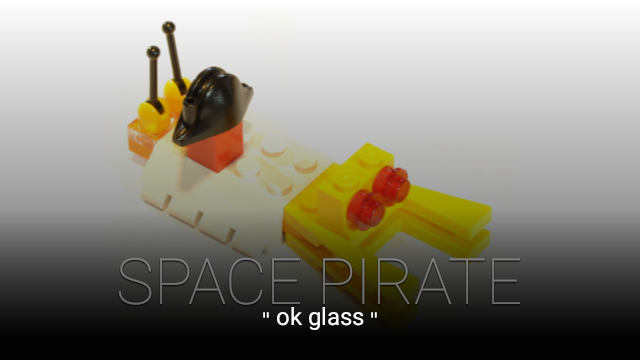
\includegraphics[width=110mm]{images/demo/titleCard}
		\caption{The title card of the demo application.}
		\label{glassDemotitleCard}
	\end{figure}
	
	\begin{figure}[H]%ht!]
		\centering
		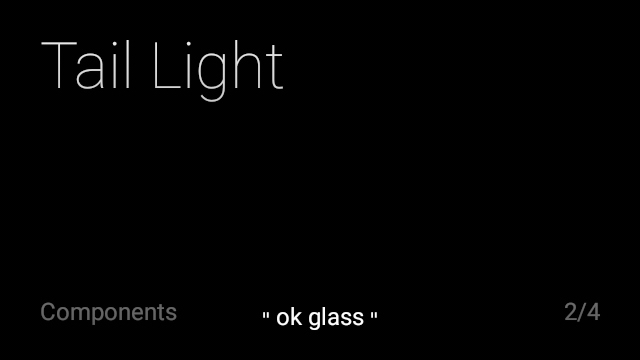
\includegraphics[width=110mm]{images/demo/componentText}
		\caption{A component slide from the demo application.}
		\label{glassDemoQR}
	\end{figure}
	
	\begin{figure}[H]%ht!]
		\centering
		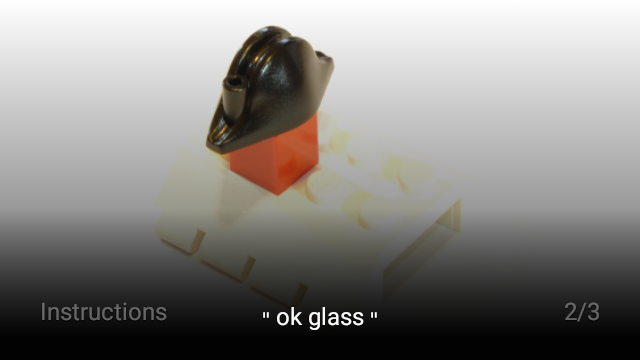
\includegraphics[width=110mm]{images/demo/instructionImage}
		\caption{An instruction slide from the demo application.}
		\label{glassDemoQR}
	\end{figure}
	
	\begin{figure}[H]%ht!]
		\centering
		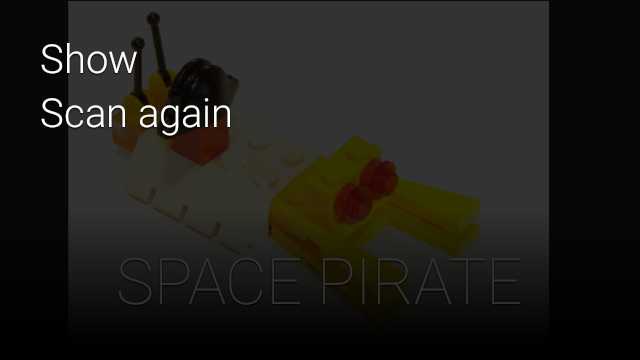
\includegraphics[width=110mm]{images/demo/voiceCommand1}
		\caption{The voice command menu in the demo application.}
		\label{glassDemoQR}
	\end{figure}

